\chapter{Benchmarking}

\label{chapter:Benchmarking}

% ----------------

In a previous work \cite{gaillardlarge}, we designed a new framework to benchmark reverse image search engines. Our approach is based on the evaluation measures of information retrieval systems described in \cite{manning2008introduction}. We model the reverse image search engine as an information retrieval system that returns an unranked set of documents for a query. If many documents are retrieved, the user is in charge of choosing the one that best suit his needs.

\section{Metrics}

\subsection{Effectiveness}
To process a query, the reverse image search engine order the indexed images by relevance. Results are retrieved using a fixed-radius nearest neighbor search. Thus, each image, whether relevant for the query or not, can be retrieved or not. This notion can be made clear by examining the following contingency table \ref{table:contingency_table}.

\begin{table}[h]
\centering
\caption{Contindency table for information retrieval from \cite{manning2008introduction}}
\label{table:contingency_table}
\begin{tabular}{|c|c|c|}
\hline
              & Relevant            & Non-relevant        \\
\hline
Retrieved     & True positive (tp)  & False positive (fp) \\
\hline
Not retrieved & False negative (fn) & True negative (tn)  \\
\hline
\end{tabular}
\end{table}

The effectiveness of the system is measured with the following metrics: Precision (P) is the fraction of retrieved documents that are relevant,

\[precision=\mathbb{P}(\text{relevant}|\text{retrieved})=\frac{\text{\#(relevant items retrieved)}}{\text{\#(retrieved items)}}=\frac{tp}{tp+fp}\]

Recall (R) is the fraction of relevant documents that are retrieved.

\[recall=\mathbb{P}(\text{retrieved}|\text{relevant})=\frac{\text{\#(relevant items retrieved)}}{\text{\#(relevant items)}}=\frac{tp}{tp+fn}\]

A single measure that trades off precision versus recall is the F-measure, which is the weighted harmonic mean of precision and recall: 

\begin{align*}
F=\frac{(\beta^2+1)PR}{\beta^2P+R} && F_{\beta=1}=\frac{2PR}{P+R}
\end{align*}

It is possible to change the weights in the harmonic mean of the F measure in order to tune it. This is done by changing the $\beta$ parameter. Values of $\beta < 1$ emphasize precision, while values of $\beta > 1$ emphasize recall. This is important in order to benchmark the system in accordance with its application.

\subsection{Performance}
It is important to measure the time the system need for indexing and searching. Indeed, the system should be able to index millions of images and search across them as fast as possible. The complexity of both the indexing and searching phases depends on the number of images and is not necessarily linear. Therefore, we propose to measure the indexing and searching time for a certain number of images.

\section{Protocol}
\label{chapter:Benchmarking:section:Protocol}
In order to compare the effectiveness and the speed of different image search methods, we created a comparison protocol. We choose 25,000 images from the MIRFLICKR dataset\footnote{http://press.liacs.nl/mirflickr}.

To be able to calculate automatically the precision and recall of the results, we applied 6 small modifications on each image, that gave us a dataset with 175 000 images. We measured the index and search speed as well as the results precision and recall.

The modifications (illustrated on Figure \ref{fig:protocol_modifications}) applied on the images are: 

\begin{enumerate}
\item Gaussian blur ($r=4$, $\Sigma=2$)
\item Black and white transformation
\item Resize to half height and width
\item JPEG compression with $quality=10$
\item Clockwise rotation by 5 degrees
\item Crop by 10\% at the right side of the image. 
\end{enumerate}

\begin{figure*}
	\centering
	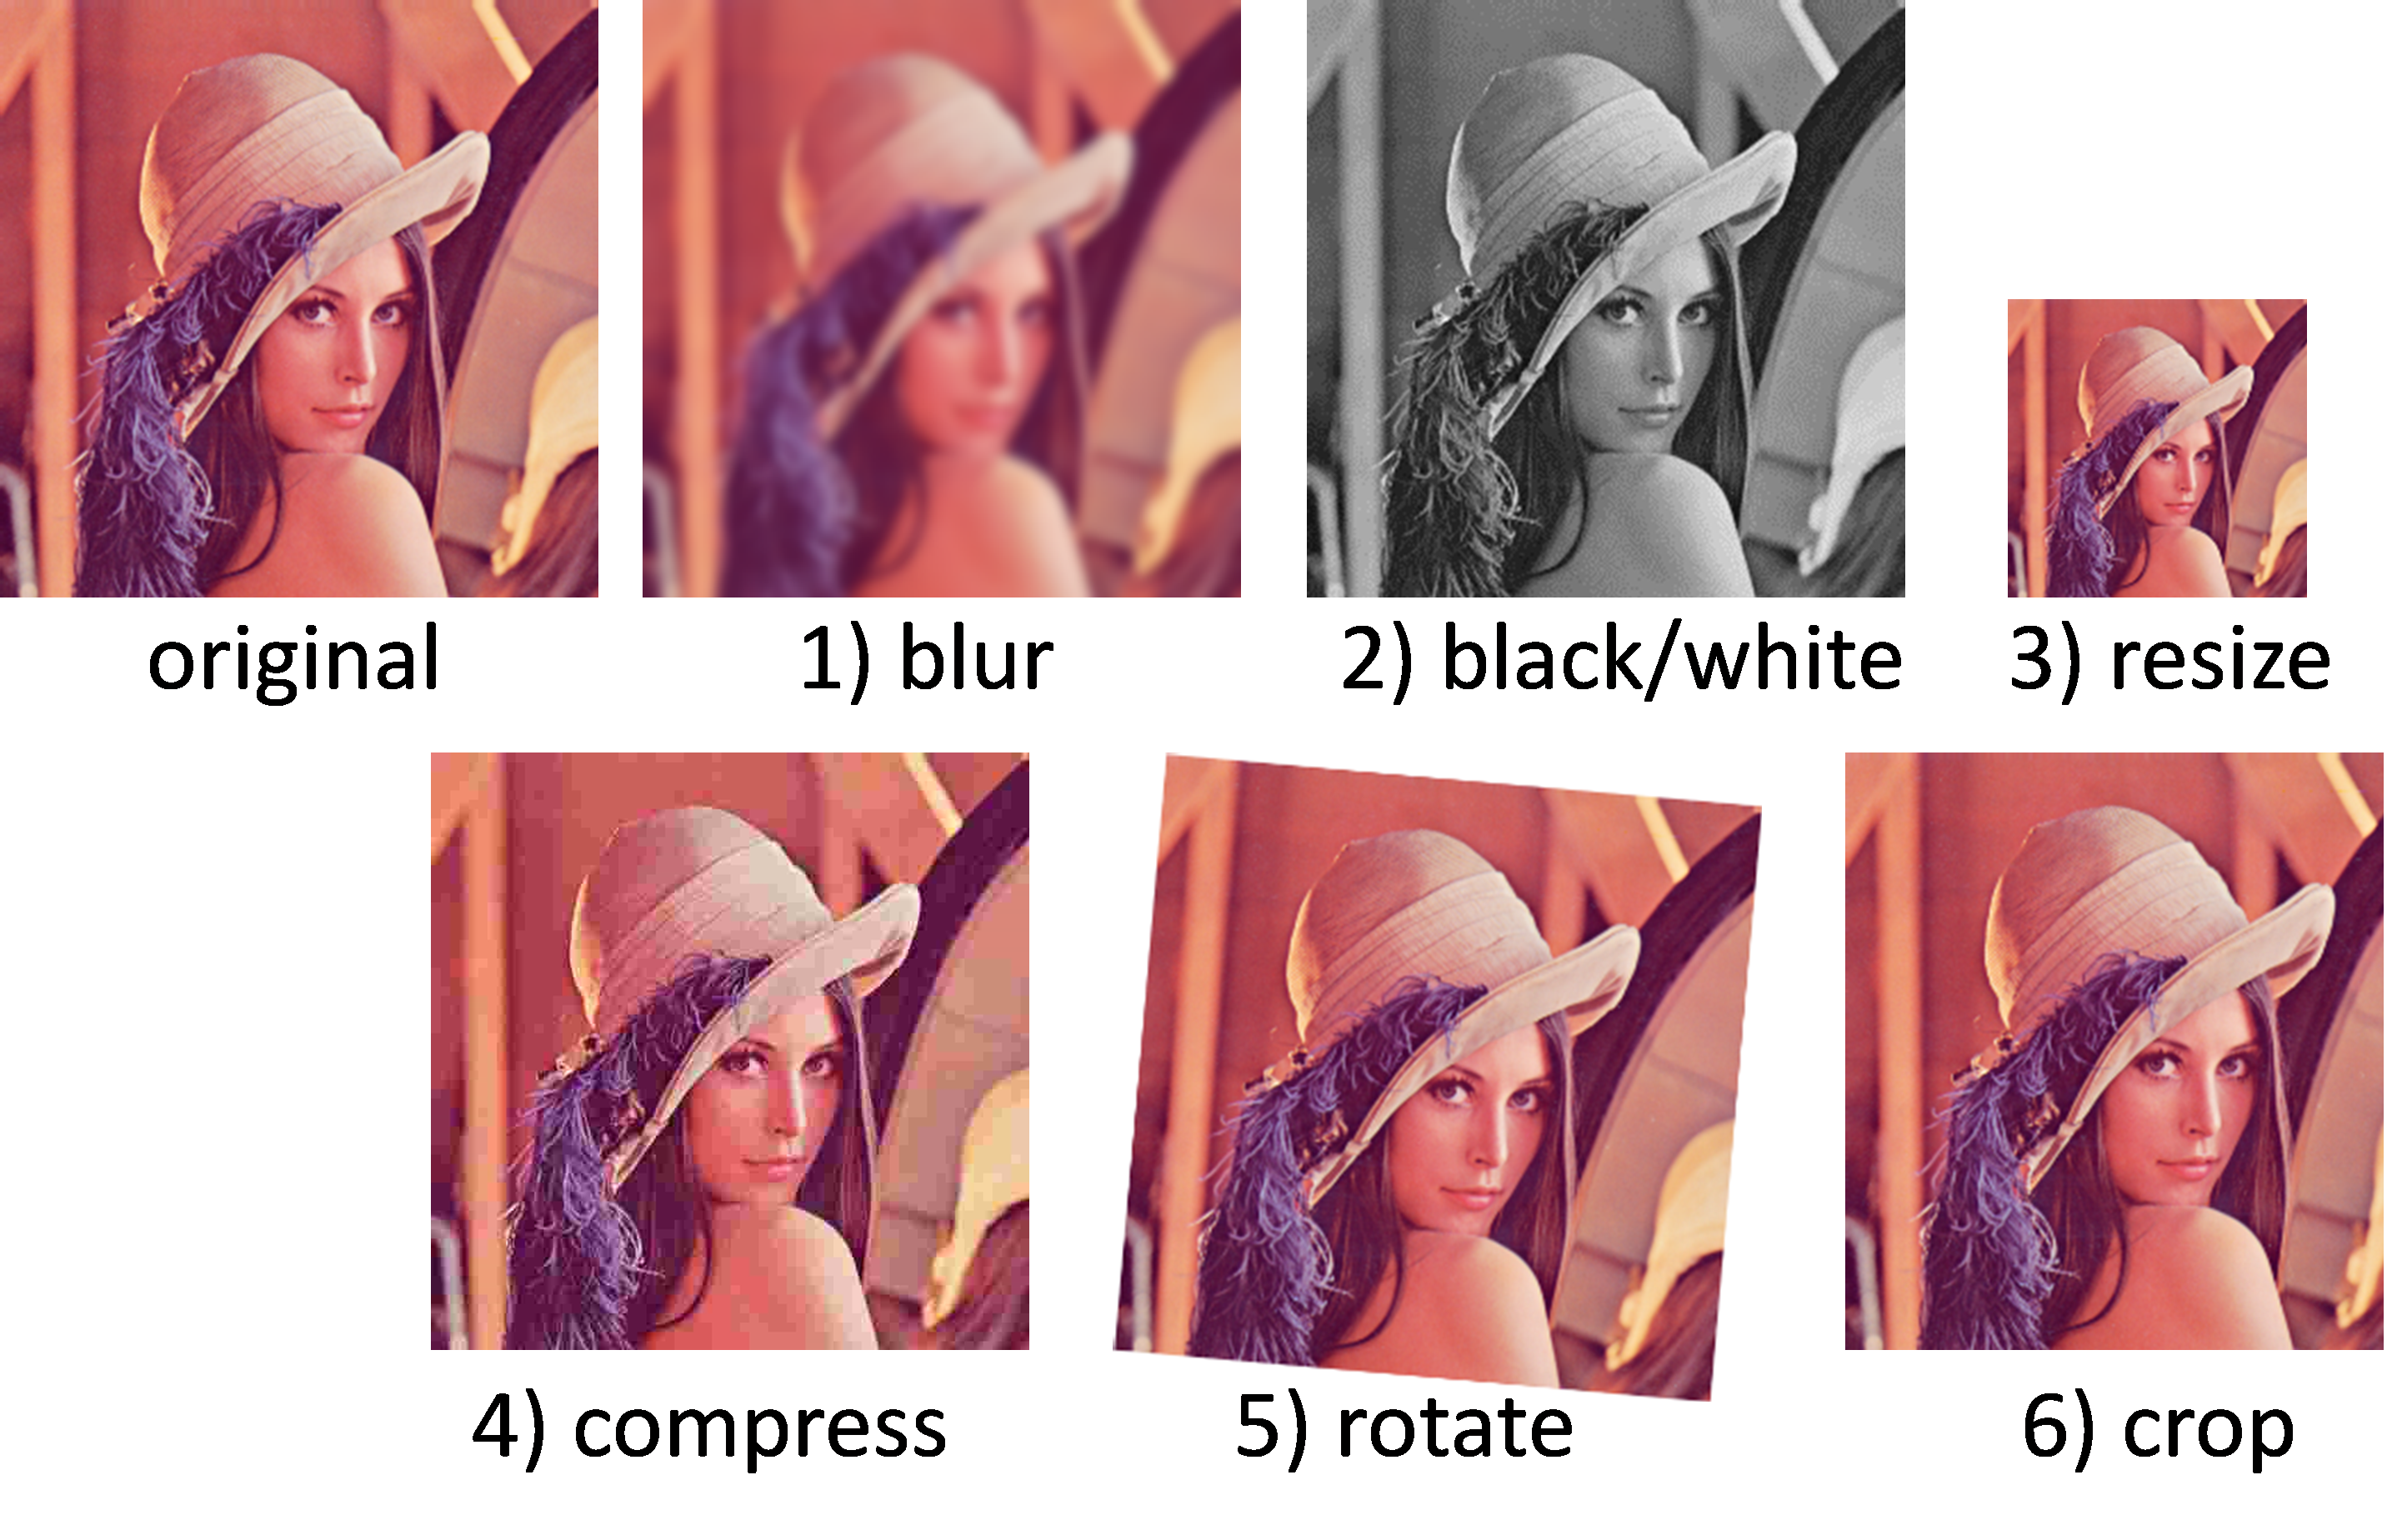
\includegraphics[width=\textwidth]{img/modifications.png}
	\caption{Illustration of the image modifications.}
	\label{fig:protocol_modifications}
\end{figure*}

These modifications represent the basic cases of small changes images usually undergo over the web. The benchmark is programmed so that it is easy to change the set of modifications.

Our benchmark protocol for a generic reverse image search engine is detailed in this section. 

\begin{enumerate}
	\item Select $N+M$ images that are representative to an application with no duplicated images. In our case $N=24,000$ and $M=1,000$ (the first 1,000 images from the dataset in alphabetical order)
	\item Split them into 2 sets of $N$ base images and $M$ non-indexed images.
	\item Select $K$ modifications and from the $N$ base images, generate $K$ new image sets containing $K \times N$ modified images. In our case $K=6$, and the modifications are those enumerated above.
	\item Index the $N$ base images and the $K \times N$ modified images according to the image representation method.
	\item Make search queries with:
		\begin{enumerate}
			\item The $M$ images from the non-indexed image set,
			\item The $N$ images from the base image set.
			\item The $K \times N$ images from the modified sets.
		\end{enumerate}
	\item Analyse the search results and compute the mean precision, the mean recall and the mean F-measure of all queries.
	\begin{enumerate}
		\item For the $M$ images of the non-indexed set, there should be no relevant result image. Thus, the result should be empty.
		\item When querying with one of the other $(K+1)\times N$ already indexed images, the relevant results are the $K+1$ images that are the modified version of the query image. Thus, the result of each query should contain K+1 images that come from the same base image as the query image.
	\end{enumerate}
\end{enumerate}

Because our system use a fixed-radius nearest neighbor search, we model it as an information retrieval system that returns an unranked set of documents. To determine the best radius, we repeat this protocol for several different radii.

It is possible to use the protocol in two different ways. Firstly, by applying all modifications to have an overview of the performances of a method. Thus, it is possible to compare two methods according to a complete workload. Secondly, by applying a single modification, for example to identify the strength and weakness of a method according to some modifications.

We implemented the protocol \footnote{See our implementation on: https://github.com/mgaillard/pHashRis} as Linux shell commands and C++, using online available libraries.

\section{Results}
\label{chapter:Benchmarking:section:Results}
We evaluate the methods described in chapter \ref{chapter:PerceptualHashing}: DCT, MH and RV based perceptual hash functions from \cite{zauner2010implementation}. 

\subsection{Retrieval performance against single modification}
We index the $N$ base images and then make $K$ search queries each with one of the $N$ modified images. We compute the F-measure for various radius and take the maximum.

\begin{figure*}
	\centering
	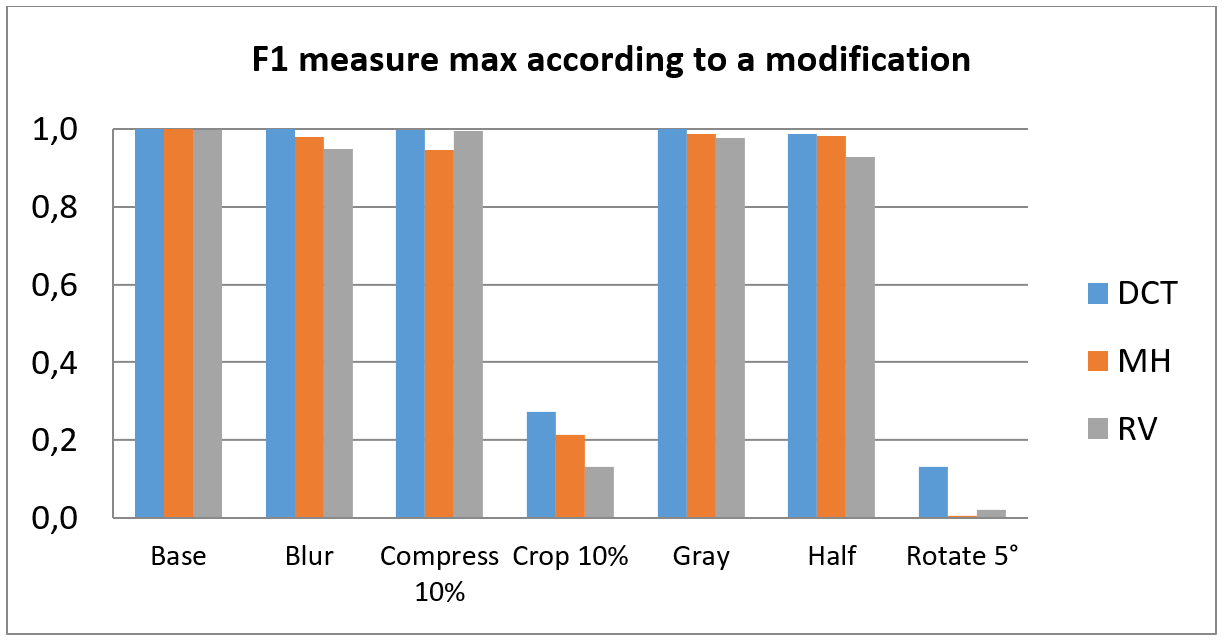
\includegraphics[width=\textwidth]{img/benchmark_single.png}
	\caption{Maximum F1-measure of DCT, MH and RV perceptual hash functions against single modifications.}
	\label{fig:benchmark_single}
\end{figure*}

The functions are robust against Gaussian blur ($r=4$, $\Sigma=2$), JPEG compression (quality 10\%), grayscale filter, and scale to half the size. However the functions are not robust against crop (10\% on the right) and rotate (5 degrees clockwise) modifications as illustrated on Figure \ref{fig:benchmark_single}.

We also tested, the evolution of our accuracy measures with different degrees of the modifications. We noticed that the different hash methods were quite sensible to rotations (above 2 degrees) or to cropping (above 5\%), but resisted very well to compression, blur or resize.

\subsection{Retrieval performance against all modifications}
To evaluate the speed and retrieval performance of a reverse image search engine, we run the protocol described in the previous section. The results are in figures \ref{fig:benchmark_dct}, \ref{fig:benchmark_mh}, \ref{fig:benchmark_rv}. We can see that all functions have equivalent retrieval performances with a maximum F-measure of about 60%.

The results (table \ref{table:benchmark_times}) showed that the DCT based hash function is clearly faster than the Marr-Hildert (MH) Operator and Radial Variance (RV) based hash functions. It is also more accurate against the 6 chosen modifications. We evaluate the retrieval performance, calculating the mean precision, recall and F-measure of the returned results. The calculation is repeated for different radius values. The radius here is a normalized distance value, below which two images are considered as similar.

The performance is evaluated through the index and search speed. Table \ref{table:benchmark_times} presents the measurements done for 125,000 images on an OVH dedicated virtual machine equipped with an Intel Xeon Haswell 8 cores at 3.1 GHz and 30 GB of RAM.

\begin{figure*}
	\centering
	\begin{tabular}{|c|c|c|}
		\hline
				& Index 125k images   & 125k queries on 125k images \\
		\hline
		DCT & 3 min 55 sec        & 3 min 59 sec                \\
		\hline
		MH  & 31 min 13 sec       & 32 min 20 sec               \\
		\hline
		RV  & 1 min 48 sec        & 3h 47 min 31 sec            \\
		\hline
	\end{tabular}
	\caption{indexing and search time measures for the DCT, MH and RV based perceptual hash functions}
	\label{table:benchmark_times}
	
	\includegraphics[width=\textwidth]{img/benchmark_dct.png}
	\caption{Precision/Recall/F-measure curves of the DCT based perceptual hash function search results according to different radius values}
	\label{fig:benchmark_dct}
\end{figure*}

\begin{figure*}
	\centering
	\includegraphics[width=\textwidth]{img/benchmark_mh.png}
	\caption{Precision/Recall/F-measure curves of the Marr-Hilderth based perceptual hash function search results according to different radius values}
	\label{fig:benchmark_mh}
	
	\includegraphics[width=\textwidth]{img/benchmark_rv.png}
	\caption{Precision/Recall/F-measure curves of the Radial Variance based perceptual hash function search results according to different radius values}
	\label{fig:benchmark_rv}
\end{figure*}